\documentclass{article}
\usepackage{tikz}
\usetikzlibrary{arrows.meta, decorations.pathmorphing, calc}

\definecolor{conductionblue}{RGB}{220, 235, 252}
\definecolor{valencegreen}{RGB}{225, 245, 225}
\definecolor{electronred}{RGB}{215, 48, 39}
\definecolor{holeblue}{RGB}{44, 123, 182}

\begin{document}

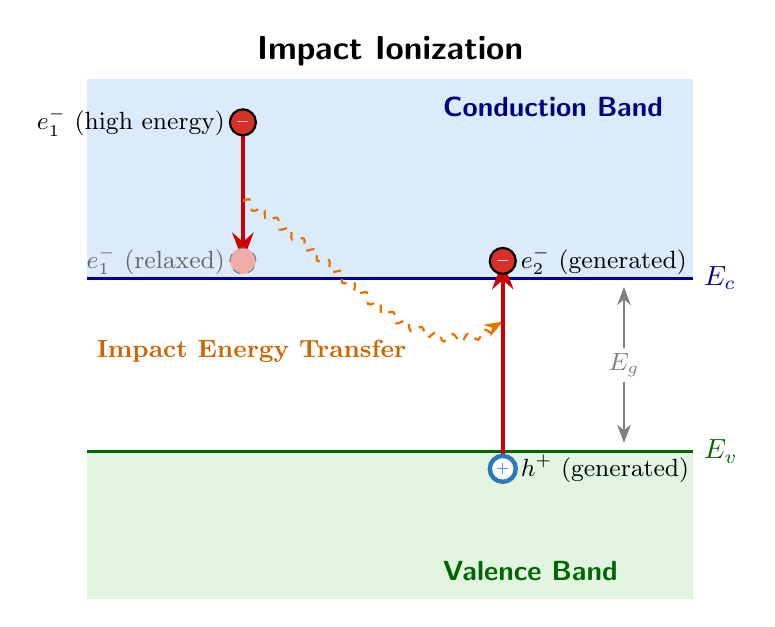
\begin{tikzpicture}[scale=1.1, >=Stealth]

    % ==========================================
    % 1. ENERGY BANDS & SHADING
    % ==========================================
    % Conduction Band (CB)
    \fill[conductionblue] (0, 2.5) rectangle (7, 4.8);
    \draw[very thick, blue!60!black] (0, 2.5) -- (7, 2.5) node[right, font=\bfseries] {$E_c$};
    \node[anchor=north west, font=\bfseries\sffamily, color=blue!50!black] at (4, 4.7) {Conduction Band};

    % Band Gap Label
    \draw[<->, thick, gray] (6.2, 0.6) -- (6.2, 2.4) node[midway, fill=white, inner sep=2pt, font=\small] {$E_g$};

    % Valence Band (VB)
    \fill[valencegreen] (0, -1.2) rectangle (7, 0.5);
    \draw[very thick, green!40!black] (0, 0.5) -- (7, 0.5) node[right, font=\bfseries] {$E_v$};
    \node[anchor=south west, font=\bfseries\sffamily, color=green!40!black] at (4, -1.1) {Valence Band};

    % ==========================================
    % 2. PARTICLES & TRANSITIONS
    % ==========================================

    % --- Process 1: High-Energy Electron Relaxation (Left side) ---
    % Initial High-Energy Electron (e1*)
    \coordinate (e1_init) at (1.8, 4.3);
    % Final Relaxed Electron (e1)
    \coordinate (e1_final) at (1.8, 2.7);

    % Relaxation transition arrow
    \draw[->, ultra thick, red!80!black] (e1_init) -- (e1_final);

    % Initial high-energy electron marker
    \draw[fill=electronred, draw=black, thick] (e1_init) circle (0.15) node[white, font=\tiny\bfseries] {$-$};
    \node[left=3pt, font=\small] at (e1_init) {$e_1^-$ (high energy)};

    % Final relaxed electron marker
    \draw[fill=electronred!40, draw=gray, dashed] (e1_final) circle (0.15);
    \node[left=3pt, font=\small, color=gray!80!black] at (e1_final) {$e_1^-$ (relaxed)};


    % --- Energy Transfer (Curved Wavy / Dashed Arrow) ---
    \draw[->, thick, dashed, orange!90!black, decorate, decoration={snake, amplitude=1.5pt, segment length=6pt}] 
        (1.8, 3.4) to[out=-30, in=-150] (4.8, 2.0);
    \node[below, font=\small\bfseries, color=orange!80!black] at (1.9, 1.9) {Impact Energy Transfer};


    % --- Process 2: Pair Generation (Right side) ---
    % Initial Valence Electron (e2) in VB
    \coordinate (e2_init) at (4.8, 0.3);
    % Final Generated Electron (e2) in CB
    \coordinate (e2_final) at (4.8, 2.7);

    % Generation transition arrow
    \draw[->, ultra thick, red!80!black] (e2_init) -- (e2_final);

    % Initial state hole creation marker (Hole left behind)
    \draw[fill=white, draw=holeblue, ultra thick] (e2_init) circle (0.15) node[holeblue, font=\tiny\bfseries] {$+$};
    \node[right=3pt, font=\small] at (e2_init) {$h^+$ (generated)};

    % Final generated electron marker in CB
    \draw[fill=electronred, draw=black, thick] (e2_final) circle (0.15) node[white, font=\tiny\bfseries] {$-$};
    \node[right=3pt, font=\small] at (e2_final) {$e_2^-$ (generated)};

    % ==========================================
    % 3. TITLE / CAPTION
    % ==========================================
    \node[anchor=north, font=\large\bfseries\sffamily] at (3.5, 5.4) {Impact Ionization};

\end{tikzpicture}

\end{document}
